\documentclass{article}
\usepackage{enumitem}
\usepackage[cachedir=minted_cache]{minted}
\usepackage{graphicx}
\graphicspath{ {./img/} }
\usepackage[margin=1in]{geometry} %used to set the margins
\setcounter{secnumdepth}{0} %used to get rid of section numbers
\title{Lab 10: Graph Traversals}
\author{Michael Morikawa}
\date{\today}


\begin{document}
\maketitle
\section{Lab Questions}
\begin{enumerate}[label=\textbf{Question \arabic*}]
    \item Does DFS or BFS guarantee to visit the vertices in a certain order?
          Why or why not? \\
          \textbf{
              DFS and BFS will of course have a different order that they visit
              the vertices but they should visit the vertices in same order every time.
              However, the order that the different searches visit the vertices depends on
              the implemention of the algoritms and the graph.
          }
    \item What is a DAG? Give an example of a real-life DAG.\\
          \textbf{
              A DAG is a directed acyclic graph, which is a digraph that has no cycles in it,
              meaning that for every vertex in the graph there is not path that leads back to
              itself. An example of a DAG would be a dependency graph that could be used for
              scheduling. In the dependency graph the vertices would be a task, the incoming edges
              are from the dependent task and the outgoing edges connect to tasks that depend on that
              vertex.
          }


\end{enumerate}

\section{Source Code}

\subsection{main.cpp}
\inputminted{c++}{../src/main.cpp}

\subsection{DFS.h (Given)}
\inputminted{c++}{../include/DFS.h}

\subsection{LabDFS.hpp}
\inputminted{c++}{../include/LabDFS.hpp}

\subsection{BFS.hpp}
\inputminted{c++}{../include/BFS.hpp}

\section{Output}
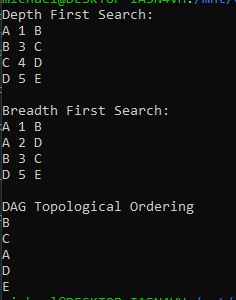
\includegraphics[]{output.png}

\end{document}